\documentclass[oneside,14pt,a4paper]{extreport}

% LANGUAGE
\usepackage[T2A]{fontenc}
\usepackage[utf8]{inputenc}
\usepackage[english, ukrainian]{babel}

% \usepackage{minted}
\usepackage{pgfplots}

% VARIABLES
\newcommand \labno    {4}
\newcommand \course   {Організація наукових досліджень}
\newcommand \group    {11}
\newcommand \lecturer {Ізонін І. В.}
\newcommand \theme    {Вибір надійного наукового видання для опублікування результатів наукових досліджень (сервіс \flqq{}Journal Finder\frqq{} від видавництва Elsevier, РЕЄСТР наукових фахових видань України)}
\newcommand \purpose  {Навчитися шукати, обирати та обґрунтовувати вибір періодичного наукового видання для опублікування результатів наукових досліджень (українські та закордонні наукові видання).}

% PACKAGES
\usepackage{amssymb}
\usepackage{amsmath}
\usepackage{multirow}
\usepackage{url}
\usepackage[unicode=true]{hyperref}
\usepackage{hanging}

% GEOMETRY
\usepackage{geometry}
\geometry{left   = 2.5cm}
\geometry{right  = 1cm}
\geometry{top    = 2cm}
\geometry{bottom = 2cm}
\renewcommand {\baselinestretch} {1.5}
\setlength\parindent{1cm}

% IMAGES
\usepackage{graphicx}
\usepackage{indentfirst}
\graphicspath{ {./imgs/} }
\usepackage{float}

% FOOTER
\usepackage{fancyhdr}
\fancyhf{}
\renewcommand{\headrulewidth}{0pt}
\cfoot{\hfill \thepage}
\pagestyle{fancy}

% CHAPTERS

\newcommand\Section[1]{
 \refstepcounter{section}
 \section*{
  \arabic{section}. #1}
}

\newcommand\Subsection[1]{
 \refstepcounter{subsection}
 \section*{
  \arabic{section}.\arabic{subsection}. #1}
}

\sloppy
\begin{document}
\begin{titlepage}

\centering
 \textbf{
  МІНІСТЕРСТВО ОСВІТИ І НАУКИ УКРАЇНИ \
  НАЦІОНАЛЬНИЙ УНІВЕРСИТЕТ \flqq{}ЛЬВІВСЬКА ПОЛІТЕХНІКА\frqq{} \
  ІНСТИТУТ КОМП’ЮТЕРНИХ НАУК ТА ІНФОРМАЦІЙНИХ ТЕХНОЛОГІЙ
 }

\vspace{0.5cm}
 \textbf{
  Кафедра систем штучного інтелекту
}

\vspace*{\fill}

  {
    \centering
    
\includegraphics[width=7cm]{imgs/logo.eps}
  }

\vspace{1cm}

  {\textbf{ЗВІТ} \par{}
  {про виконання практичної роботи №\labno}
   \par}
  {з курсу \flqq{}\course\frqq{} \par}

\vspace{1cm} \theme

\raggedleft\vfill

 {\textbf{Виконав:} \par}
 {ст. гр. КНСШ-\group \par}
 {Тимошенко Павло Олександрович \par}

% \vspace{1cm}

 {\textbf{Перевірив:} \par}
 {доцент каф. СШІ, к.т.н.,}
 {\lecturer \par}

\vspace{1cm}

\centering {Львів -- \the\year \par}

\end{titlepage}

\Section{Постановка завдання}

Далі описано пункти, які потрібно виконати у межах цієї практичної роботи.

\begin{enumerate}
    \item Написати назву, анотацію та ключові слова статті англійською та українською мовами.
    \item З використанням сервісу \flqq{}Journal Finder\frqq{} від видавництва Elsevier здійснити пошук релевантних журналів для опублікування статті англійською мовою. Подати (наприклад у вигляді таблиці) на менше п'яти різних журналів із основними їхніми показниками (імпакт-фактор, квартиль, тривалість рецензування, відсоток прийнятих статей, інші). Обрати один із журналів для опублікування результатів, та обґрунтувати вибір.
    \item З використанням сервісу \flqq{}РЕЄСТР наукових фахових видань України\frqq{} здійснити пошук релевантних журналів з технічних наук для опублікування статті українською мовою. Подати (у вигляді таблиці) не менше п'яти різних журналів із основними їхніми показниками (категорія видання, індексація наукометричними базами, вартість публікації, кількість випусків у рік, інші). Обрати один із журналів для опублікування результатів наукових досліджень та обґрунтувати свій вибір.
    \item Здійснити опис проведеної роботи.
\end{enumerate}

\Section{Хід роботи}

В цьому розділі описано процес виконання практичної роботи та пророблені кроки. 

\Subsection{Опис роботи}

\textbf{Назва дослідження (укр.)}: Використання та оптимізація алгоритму Вітербі при визначення частин мови в тексті українською.

\textbf{Назва дослідження (англ.)}: Use and improvenemts of Viterbi algorithm in POS tagging in Ukrainian language.

\textbf{Ключові слова (укр.)}: алгоритм Вітербі, обробка мови, розмітка частин мови, українська мова.

\textbf{Ключові слова (англ.)}: Viterbi algorithm, NLP, POS tagging, Ukrainian language.

\textbf{Анотація (укр.)}: У роботі розкрито застосовність алгоритму Вітербі до текстів українською при вирішення проблеми розмітки частин мови, а також перевірено його надійність. Також розроблено надійний та швидкий спосіб використання алгоритму на даних, яких не було в тренувальному наборі. Виявлено недоліки алгоритму та продемонстровано можливі способи оптимізації.

\textbf{Анотація (англ.)}: This paper reveales use of Viterbi algorithm in POS tagging of texts in Ukrainian. Also robust and reliable way of the algorithm use on unknown-at-training-stage data was developed. The shortcomings of the algorithm are revealed and possible ways of optimization are demonstrated.

\Subsection{Пошук в Journal Finder}

За наведеним описом у Journal Finder\cite{finder} мені вдалося знайти лише три журнали для публікації. Процес пошуку показано на Рис.~\ref{pic:journal-finder}. Дані про них подано у Табл.~\ref{tab:journal-finder}. За отриманою назвою я також знайшов ці журнали у SJR\cite{sjr} журналі, і дізнався квартилі. Журнал, знайдений у SJR, показано у ~\ref{tab:scimagojr}. У таблиці подано квартиль лише за попередній рік (2020).

\begin{table}[H]
\centering
\begin{tabular}{p{4cm}|p{2cm}@{}p{3cm}@{}p{3cm}@{}p{1cm}@{}ll}
Назва                                       & \rotatebox{90}{Імпакт-фактор} & \rotatebox{90}{Квартиль} & \rotatebox{90}{Тривалість реценз.} & \rotatebox{90}{Відсоток прийнятих статей} & \rotatebox{90}{CiteScore} & \rotatebox{90}{Час публікації} \\ \hline
Computer Speech and Language                & 1.899         & Theoretical Computer Science & 13 тижнів          & 23\%                      & 6.9       & 5 тижнів       \\
Journal of Infometrics                      & 5.107         & -- & 4 тижні            & 15\%                      & 8.6       & 4 тижні        \\
Journal of Molecular Graphics and Modelling & 2.518         & Spectroscopy & 3 тижні            & 23\%                      & 3.9       & 3 тижні        \\
\end{tabular}
\caption{Статті, знайдені за допомогою JournalFinder}
\label{tab:journal-finder}
\end{table}

\begin{figure}[H]
\centering
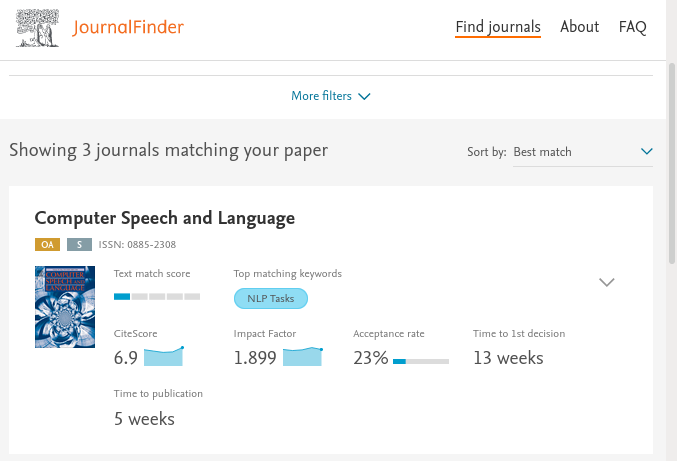
\includegraphics[width=\textwidth]{imgs/sp4_journal_finder.png}
\caption{Пошук журналів у Journal Finder.}
\label{pic:journal-finder}
\end{figure}

\begin{figure}[H]
\centering
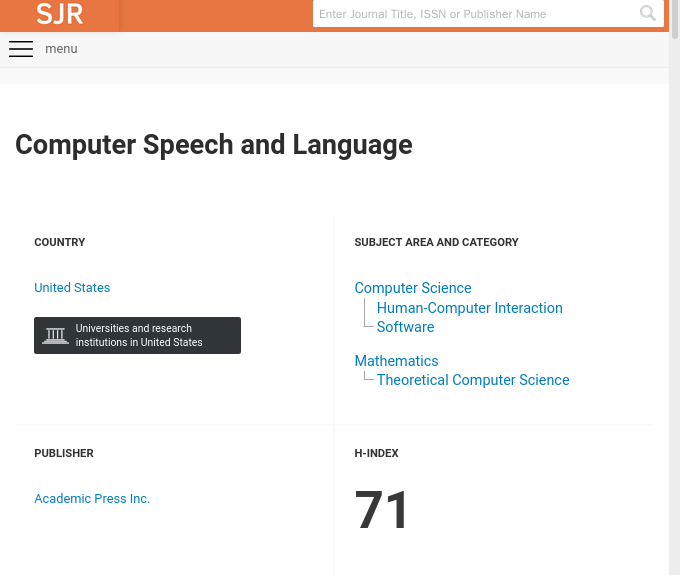
\includegraphics[width=\textwidth]{imgs/sp4_scimagojr.png}
\caption{Пошук деталів про журнал у SJR.}
\label{pic:scimagojr}
\end{figure}

Для публікації власного дослідження я би обрав журнал \flqq{}Computer Speech and Language\frqq{}, оскільки він найбільше відповідає тематиці роботи. \flqq{}Journal of Infometrics\frqq{} не підходить для публікації тому, що у ньому подаються статті, які досліджують \flqq{}проблеми інфометрики, використовуючи методи з інших областей таких, як математика, статистика, комп'ютерні науки, економіки [...]\frqq{}\footnote{Цитата з опису журналу.}, а невідповідність третього журналу зрозуміла з самої лише назви.

\Subsection{Пошук у РЕЄСТРі}

Оскільки у РЕЄСТРі\cite{rejstr} відсутні можливість шукати за ключовими словами, у параметрах розширеного пошуку я обрав технічну галуз науки і спеціальність \flqq{}122 Комп'ютерні науки\frqq{}. Результатів вийшло небагато, тож я зміг прогортати усі журнали вручну, і обрати щось на потрібну тематику. Процес пошуку продемонстровано на Рис.~\ref{pic:rejestr}. Список обраних показано у Табл.~\ref{tab:rejestr}. Однією з мов повного тексту для усіх поданих журналів є українська. На сайті РЕЄСТРу та на сайті самих журналів відсутня інформація про вартість публікації, тож ці дані не приведено в таблиці.

\begin{figure}[H]
\centering
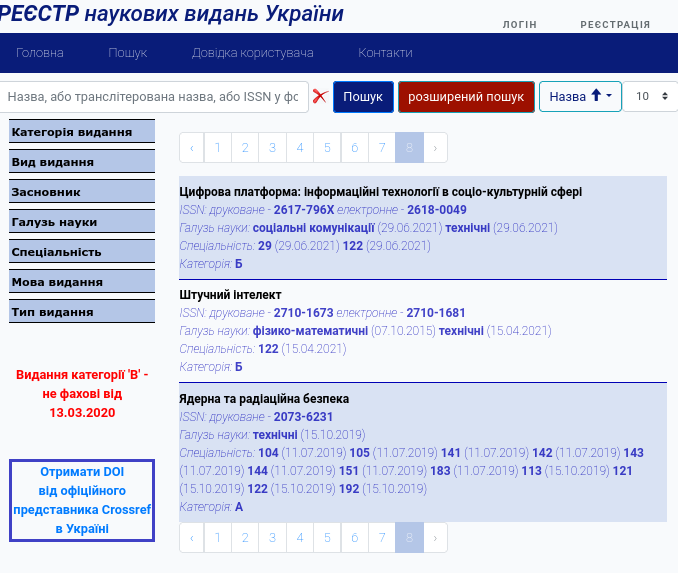
\includegraphics[width=\textwidth]{imgs/sp4_rejestr.png}
\caption{Пошук журналів у РЕЄСТРі.}
\label{pic:rejestr}
\end{figure}

\begin{table}[H]
\centering
\begin{tabular}{llp{2cm}}
Назва                        & Індексація                     & Випусків у рік \\ \hline
Технічні науки та технології & Google Scholar, CrossRef       & 4              \\
Штучний інтелект             & Google Scholar                 & 4              \\
Наука та іновації            & Google Scholar, CrossRef, ESCI & 6              \\
Проблеми програмування       & Google Scholar                 & 4              \\
Математичні машини і системи & Google Scholar                 & 4             
\end{tabular}
\caption{Статті, знайдені за допомогою РЕЄСТРу.}
\label{tab:rejestr}
\end{table}

Серед усіх поданих журналів для публікації я би обрав \flqq{}Штучний інтелект\frqq{} тому, що його тематика найбільше відповідає тематиці роботи: \textit{\flqq{}Концептуально-теоретичні проблеми штучного інтелекту і моделювання, [...], природномовні системи [...]\frqq{}}.

\Section{Результати та висновки}

У цій практичній роботі я шукав журнали, релевантні до тематики наукового дослідження. Пошук виконувався за допомогою JournalFinder та РЕЄСТРу наукових видань України за відповідною тематикою та ключовими словами. Серед знайдених журналів я обрав той, який підходив найбільше.

У каталозі JournalFinder я знайшов 3 журнали, лише один з яких відповідав тематиці дослідження. Якби таких журналів було би більше, можна було би обрати найвідповідніший за відсотком прийнятих статей, тривалістю прийняття та публікації, а також коефіцієнтом впливу (Impact Factor).

Здобуті навички можна використати для пошуку журналу, в якому можна опублікувати власне дослідження.

\Section{Список використаної літератури}

\begingroup
\renewcommand{\section}[2]{}
\renewcommand{\chapter}[2]{}
\begin{thebibliography}{99}
\bibitem{rejstr} Реєстр наукових видань України [Електронний ресурс] // Реєстр наукових видань України. – Режим доступу: \url{http://nfv.ukrintei.ua/search} (дата звернення: 08.11.2021). – Назва з екрана.
\bibitem{finder} Elsevier® JournalFinder [Електронний ресурс] // Elsevier® JournalFinder. – Режим доступу: \url{https://journalfinder.elsevier.com/} (дата звернення: 08.11.2021). – Назва з екрана.
\bibitem{sjr} Scimago Journal Rankings [Електронний ресурс] // Scimago Journal \& Country Rank. – Режим доступу: \url{https://www.scimagojr.com/journalrank.php} (дата звернення: 08.11.2021). – Назва з екрана.
\end{thebibliography}

\end{document}
